\documentclass[a4paper, 11pt]{article}
\setlength{\topmargin}{-0.5in}
\setlength{\textheight}{9.5in}
\setlength{\oddsidemargin}{-.1in}
\setlength{\textwidth}{6.5in}
\usepackage{graphicx}
\graphicspath{ {images/} }
\usepackage{datetime}

\begin{titlepage}

\LARGE\title{Real Time Tempo Analysis of Drum Beats}

\LARGE\author{Author: \textbf{Philip Hannant}, Supervisor: \textbf{Professor Steve Maybank}}



\end{titlepage}

\begin{document} 

\maketitle
\newpage
\tableofcontents
\clearpage

\maketitle{} \section{Introduction \& Background}
Having played the drums for nearly twenty years I have experienced a number of different training tools in order to improve my timing, these tools have always been exclusive to midi driven electric drum kits. These drum kits are able to include training tools within their drum modules which utilise the midi events being triggered by the player and give live feedback to the exact timing and instrument being played. An example of such a system is the Roland DT-1 V-Drums tutor which is a software package that can be connected to their V-Drum modules in order to provide the player with an interactive experience in order to help a drummer improve their rhythm, coordination sight reading. Such an extensive and accurate range of tutoring functions is only made possible by the midi events that are intrinsic to an electronic drum kits function. (an example of the GUI can be found in figure 1) [roland ref]. These tutoring tools are not however available to a drummer who does not own an electronic drum kit, they are restricted to using a metronome and using their ear to determine their timing and rhythm. To address this, I intend to investigate the current audio tempo analysis and beat tracking algorithms available solely for the purpose of being implemented within an drum tutoring software package for the use with acoustic drums.
6, 3, 7, 2, 1
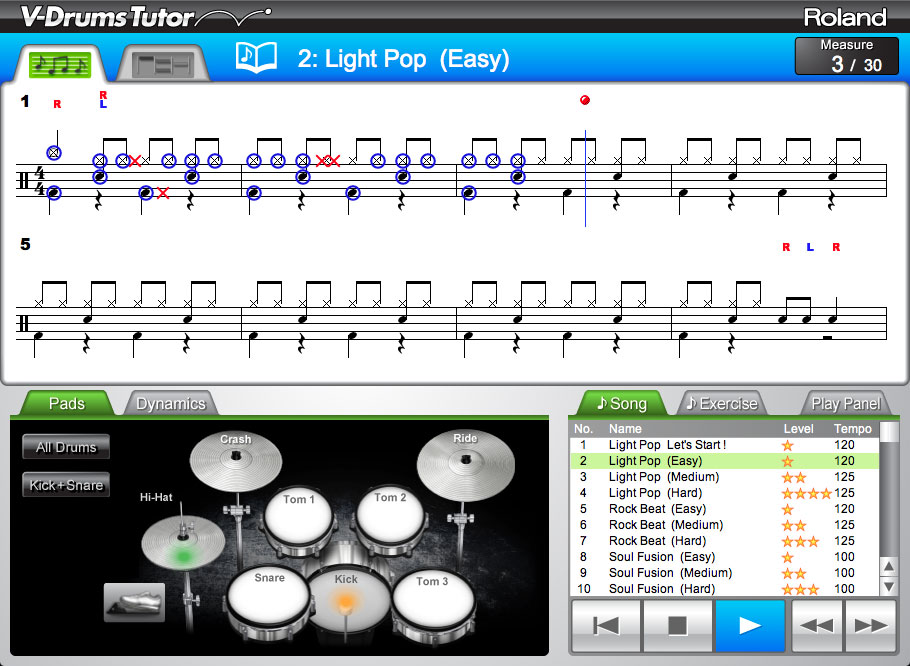
\includegraphics[scale=0.2]{dt-1_ss_main_notation_gal} 

\subsection{Beat Detection}

Detecting musical time is a skill which is not only a fundamental musical skill [1] but also something that can seemingly come naturally to humans, the majority being able to analyse and reproduce discrete metrical stuctures of a piece of music [2]. Producing algorithms to replicate this nature human ability is probably first attempted by Longuet-Higgins [1], where he began to consider that rhythm as a binary tree with each node representing a note or rest. This theory developed into a system which would use a static tolerence limit on how much a the downbeats varied and enabling the perceived tempo to be adjusted accordingly [add longuet references]. Since Longuet-Higgins first work there have been a number of different approaches to beat detection in audio, M. Goto and Y. Muraoka created a system which would learn the frequencies of the bass drum and snare drum, in order to then detect events triggered by these instruments during a piece of music [Goto \& muroaka]. In 2001 Simon Dixon presented a system which uses processed a piece of audio in order to generate a tempo hypotheses at various metrical levels, multiple agents were then employed to find the sequence of beat times which best matched the salient rhythmic events which were originally detected.

The majority of the audio beat detection systems developed to date rely on an onset detection function, where an audio onset is considered to be the beginning of each music note within a piece of music[wiki onset] and therefore can be used to find time-locations within all sonic events in a piece of music [MIREX]. 



systems developed to perform beat tracking and temporal analysis with the majority using the ``surfboard'' method first described by schloss which observed the peaks of sound energy within a piece of music in order to discern the beat locations and temporal information [schloss]. 

This method however was not considered accurate enough to fully replicate the skill of a trained musician at beat detection, it was soon recognised that onset detection would play a fundamental part in any future beat detection algorithms. Where the an indicator of a new onset is seen as ``an increase in energy (or amplitude) within some frequency band(s)'' [4].


Due to the rapidly expanding research being carried out on beat detection, in 2005 the 1st annual Music Information Retrieval Evaluation eXchange (MIREX) was held. MIREX has been set up as a contest with the goal of comparing state-of-the-art algorithms and music information retrieval [MIREX website]. The topics to be evaluated were proposed by the participants and in the first year, three of the nine topics concerned beat detection (Audio Drum Detection, Audio Onset Detection and Audio Tempo Extraction).  

Find the reference regarding how much work has been done in this field

Light version of beatroot and DWT

Needs to add history of all the work carried out on audio analysis with an emphasis on tempo detection


To date, the majority beat detection software has focused mainly on the dj industry where tempo and beat matching are popular aspects to be included in modern dj programs. There are however other sectors of the music industry would find beat detection software a useful, in particular, drummers could find it an enormously useful training tool. There are currently many systems available to a drummer, 




\subsection{Beatroot}
Beatroot is an audio beat tracking system which was first presented by Simon Dixon in the 2002 paper ``On the analysis of musical expression in audio signals''. The system is described as ``an off-line beat tracking system which finds the times of musical beats and tracks changes in tempo throughout a performance'' [dixon 2002]. Beatroot uses two interacting processes in order to process audio; 1) Tempo induction calculated from the rate of detected beats and 2)Beat tracking produced by the synchronising the pulse sequences detected within the audio signal. These processes are performed using the following steps:

\begin{enumerate}
\item The audio signal is first passed through a spectral flux onset detection function which uses the short-term Fourier transform (further detailed provided in the following section). 
\item A clustering algorithm is then employed to find all of the significant metrical units within the signal, these clusters are then compared and ranked accordingly to produce a set of tempo hypotheses.
\item A multiple agent architecture is ultised to to match the sequences of detected beats, where each agent represents a specific tempo value and alignment of beats with the audio signal.
\item Finally, the agents are then evaluated against the original hypothesised beats and the highest ranked sequence is then returned as the solution.
\end{enumerate}

\subsubsection{Spectral Flux Onset Detection}


\subsubsection{Short-Term Fourier Transform}
The Short-Term Fourier Transform (STFT) is based on the original Fourier Transform (FT) which was developed by Joseph Fourier in 1822, which can be used to find out how much of each frequency exists in a signal. The STFT was developed in order to solve provide a solution to the fact that the Fourier Transform does not work on non-stationary signals which results in it not being possible to used to find out when a frequency exists in the time-domain [polikar 2]. The STFT solved this issue by dividing the signal into a number smaller segments using a window function, which effectively created a series of stationary signals which the Fourier Transform could be successfully used on. This however did not fully solve the problem as the size of window function used had an effect on the the quality of frequency resolution and time resolution:
[polikar3]
\begin{itemize}
\item Narrow Window Function \longrightarrow  Good Time Resolution, Bad Frequency Resolution
\item Wide Window Function \longrightarrow  Bad Time Resolution, Good Frequency Resolution
\end{itemize}

This was eventually solved by development of Wavelet Transforms which are capable of providing time and frequency information simultaneously in order to give a time-frequency representation of a signal, which are described in further detail in the next section.

\subsection{Audio Analysis using the Discrete Wavelet Transform}
The Discrete Wavelet Transform (DWT) is a form of wavelet transform which foundations go back to 1976 when Crosier, Estaban and Galand devised a technique to decompose discrete time signals [polikar]. The DWT uses digital filtering techniques like the orginal Continuous Wavelet Transform, however it is significantly easier to implement. The DWT works by passing the signal through a series of high pass filters to analyse the high frequencies and low pass filters to do the same to low frequencies. The low pass filtering results in the resolution being halved but leaves the scale unchanged and the high filtering halves the time-resolution but doubles the frequency resolution, which effectively reduces the uncertainty in the frequency by half [polikar 4]. Due to this, the DWT is considered to share similar time-frequency resolution characteristics with the human ear [DWT Tzanetakis et al].

Tzanetakis, Essl and Cook described how the DWT could be used to extract information from non-speech audio, their beat detection algorithm was based on detecting the salient periodicities of the audio signal and was made up of the following steps[tzanetkis]. 

\begin{enumerate}
\item Signal decomposed into a number of octave frequency bands using DWT
\item The subsequent time domain amplitude envelope is extracted for frequency each using low pass filtering, full wave rectification and downsampling
\item Each band is then normalised
\item The envelopes of each band are then summed together and an autocorrelation function is computed
\end{enumerate}

\subsubsection{JWave}
JWave is 
Unlike the STFT based beat detection tool, Beatroot there are not currently any 

\maketitle{}
\section{Aims and Objectives}

As part of my project I propose to build a real time drumbeat tempo analyser, this will use a combination of existing libraries in order to provide a basis for the creation of a live drumming tempo training tool. I will elaborate on the key features of this work in the following sections.

 which wiill implement a variety of different wave analysis algorithms. sound energy analysis and discrete wavelet transform technologies. I will provide more details regarding the system architecture in the following sections. 

Investigate with a sole focus on drums how accurate/reliable the beatroot and discrete wavelet transform algorithms are in order to ascertain how viable a future mobile metronome and drum tempo training application would be.



\subsection{Core Project Features}
\begin{itemize}
\item Live audio capturing and processing
\item Log detailed comparative information regarding the efficiency and accuracy of the Beatroot and DWT implemntation using JWave
\item GUI to provide the user with current tempo played and notification of beat detection
\item Build and test an extensive sample set of drum beats at varying tempos and velocities in order to ensure the system is tested against as close to a real drummer as possible
\end{itemize}

\subsection{Non-Core Project Features}
\begin{itemize}
\item Live tempo status bar created and tested with a live player to demostrate the systems ability to handle varying tempos
\item Create a calibration mode within the system in order to allow for the system to learn the relevant frequencies of all of the drums being played
\item Extend GUI to provide the user with real time notification on when a certain drum is played by using the stored calibrated frequencies
\end{itemize}

\maketitle{} 
\section{Development Plan for the Solution}

The first part of this project involves the setting 

\subsection{Live Audio Processing}
In order to capture and process live audio the Javax Sound package will be ulitlised, where the audio will be captured using the Java Line hierachy; specifically the TargetDataLine class, which requires an instance of the Javax Sound AudioFormat class to be parsed in to work. The AudioFormat class is made up of a number of constructed fields which are defined as follows:

\begin{itemize}
\item Encoding - This will be set to ``''PCM.signed``'', representing audio encoded to the native linear pulse code modulation, where quantization levels are linearly uniform [wiki].
\item Sample Rate - 44,100, set to match CD quality for the number of analogs samples which will be analysed per second. 
\item Sample Size in Bits - 24, based on a sound card with a 24 bit sample depth.
\item Channels - 2, audio will be captured using a stereo microphone.
\item Frame Size - 6, where frame size equals the number of bytes in a sample multiplied by the number of channels.
\item Frame Rate - 44,100, same as sample rate.
\item Big Endian (boolean) - false, as the project will be developed on an Intel core which uses a little endian architecture. Where endianess refers to the order of bytes which make up a digital word, with big endianess storing the most significant byte at a certain memory address and the remaining bytes being stored in the following higher memory addresses. The little-endian formate reverses the order storing the least significant at the lowest and most siginicant at the highest memory address [https://en.wikipedia.org/wiki/Endianness].
\end{itemize}

\subsection{Comparative analysis of Beatroot and JWave}
A key part of this project is to ascertain whether the technologies currently available are accurate enough to create a training tool similar to the midi based software described in section 1. To achieve this the 2 libraries will need to be run in parallel with the same captured audio and a predetermined set of parameters recorded. For the tempo analysis this will simply be the bpm recorded at the end of each frame, all of the bpm's within the sample set will be exact and in order to match the current midi software packages accuracy any returned bpm's should be exact. However, very small deviations in tempo can be very hard to detect to the human ear so some margin of error will be applied. To account for the fact that at the slower bpm's any beat out of place will be a lot easier to notice than at a higher bpm, the margin for error will be weighted by using the following equation;

\[ m = bpm - 60 * 0.0001\]

where \(m\) represents the weighted value for the margin for error to be applied.

\subsection{Develop GUI \& logging system}


\subsection{Build Extensive drum sample set}
The success of this project will rely heavily on the amount of data that the system can produce and in order to do this a large set of drum beat samples will need to be created. The drum beats themselves will be created using the installed midi drumbeats with the Apple software package, Garageband. The sample set will need to contains beats from a variety of styles as well as samples with fluctuating tempos. The main aspects of the sample set can be found below:

\begin{itemize}
\item The tempo range will be 60 - 160 beats per minute (bpm), although some samples will be be created with varying tempos in order to closely reflect a real human player
\item The time signatures will be mainly in common time (4/4) to reflect playing styles, however some beats will use swing time which will either be created by feel within the sample or by using triplets with a duple meter in 12/8
\item Velocities will be varied across the sample set, accent and ghost notes will be used in line with a real playing style
\item The sample set will contain a wide range of drum beats, including; beats using one drum, those only with a back beat, beats incorporating single rests within a bar or for the whole duration of a bar \& beats with large solos and cymbal work
\end{itemize} 

Musical styles will comprise of rock \& pop, blues and jazz, with the main emphasis failing on rock \& pop beats. Each style will have between 5 - 10 unique samples created, which will in turn each sampled with a bpm value starting at 60 and increasing in steps of 5 up until the maximum, which will account for approximately 500 separate samples. There will also be a final set of simple single and multiple drum beats included which will produce another c. 10 unique samples, which will give a total sample set size of c. 750 samples.

\maketitle{} 
\section{Project Schedule}

\begin{table}[]
\caption{Project Timeline} 
\centering
\begin{tabular}{|p{4cm}|p{8cm}|}
 \hline
\textbf{Dates} & \textbf{Task}\\ [0.5ex]
\hline 
w/c 13th June & Develop live audio capturing system\\
\hline 
w/c 20th June & Set up Beatroot library in development environment\\
\hline 
w/c 27th June & Implement DWT tempo and beat detection algorithm in Scala/Java\\
\hline 
w/c 4th July & Test systems with single live audio source\\
\hline 
w/c 11th July & Develop system to store data generated during tempo analysis\\
\hline 
w/c 18th July & Research and build appropriate framework to process captured audio in parallel e.g. akka actors\\
\hline 
w/c 1st August & Create sample set of drum beats\\
\hline 
w/c 8th August & Test system using full sample set\\
\hline 
w/c 15th August & Develop UI\\
\hline 
w/c 22nd August & Analyse logged data\\
\hline 
w/c 29th August & Write up report\\
\hline 
w/c 5th September & Present findings to project supervisor\\
\hline 
w/c 12th September & Finalise report\\
\hline 
w/c 19th September & Submit report\\
\hline
\end{tabular}
\end{table}

\maketitle{} 
\section{References}
http://www.roland.co.uk/blog/exploring-roland-dt-1-v-drums-tutor-software/
https://en.wikipedia.org/wiki/Pulse-code\_modulation
http://www.jsresources.org/faq\_audio.html\#frame\_rate
https://en.wikipedia.org/wiki/Onset\_(audio)
http://www.music-ir.org/mirex/wiki/2016:Audio\_Onset\_Detection
http://users.rowan.edu/~polikar/WAVELETS/WTpart2.html

\end{document}
